% Figure from MATH 493 notes, section 50 (lecture 10/30, Jordan-Hoelder).
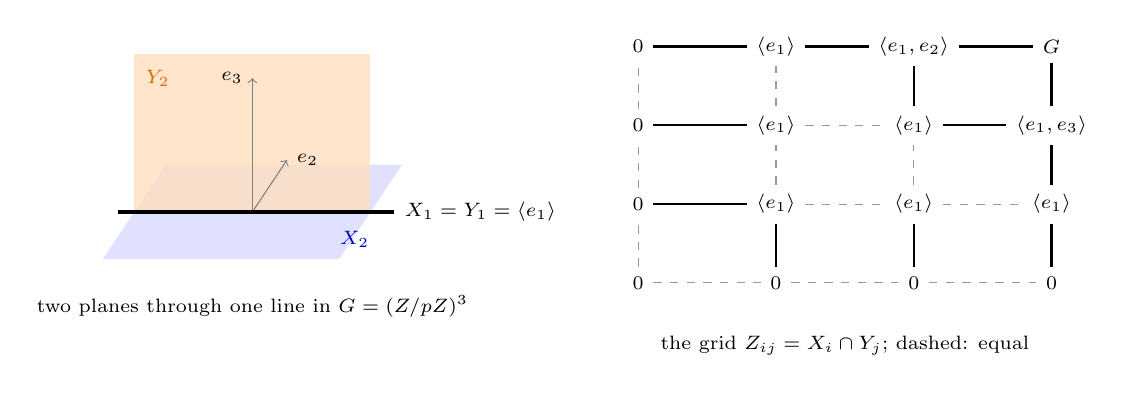
\begin{tikzpicture}[x=1cm, y=1cm]
% three-dimensional picture: X_2 = <e1, e2> (blue, horizontal), Y_2 = <e1, e3> (orange, vertical), X_1 = Y_1 = <e1>
\fill[blue!12] (-1.2,-0.7) -- (1.8,-0.7) -- (2.6,0.5) -- (-0.4,0.5) -- cycle;
\fill[orange!25, opacity=0.8] (-0.8,-0.1) -- (2.2,-0.1) -- (2.2,1.9) -- (-0.8,1.9) -- cycle;
\draw[black!50, ->] (0.7,-0.1) -- (1.14,0.56) node[right, font=\scriptsize, text=black] {$e_2$};
\draw[black!50, ->] (0.7,-0.1) -- (0.7,1.6) node[left, font=\scriptsize, text=black] {$e_3$};
\draw[black, very thick] (-1.0,-0.1) -- (2.5,-0.1) node[right, font=\scriptsize] {$X_1 = Y_1 = \langle e_1 \rangle$};
\node[blue!75!black, font=\scriptsize] at (2.0,-0.45) {$X_2$};
\node[orange!85!black, font=\scriptsize] at (-0.5,1.6) {$Y_2$};
\node[font=\scriptsize, align=center] at (0.7,-1.3) {two planes through one line in $G = (\mathbb{Z}/p\mathbb{Z})^3$};
\begin{scope}[shift={(5.6,-1.0)}, x=1.75cm, y=1.0cm]
\node[font=\scriptsize] (z00) at (0,0) {$0$};
\node[font=\scriptsize] (z01) at (0,1) {$0$};
\node[font=\scriptsize] (z02) at (0,2) {$0$};
\node[font=\scriptsize] (z03) at (0,3) {$0$};
\node[font=\scriptsize] (z10) at (1,0) {$0$};
\node[font=\scriptsize] (z11) at (1,1) {$\langle e_1 \rangle$};
\node[font=\scriptsize] (z12) at (1,2) {$\langle e_1 \rangle$};
\node[font=\scriptsize] (z13) at (1,3) {$\langle e_1 \rangle$};
\node[font=\scriptsize] (z20) at (2,0) {$0$};
\node[font=\scriptsize] (z21) at (2,1) {$\langle e_1 \rangle$};
\node[font=\scriptsize] (z22) at (2,2) {$\langle e_1 \rangle$};
\node[font=\scriptsize] (z23) at (2,3) {$\langle e_1, e_2 \rangle$};
\node[font=\scriptsize] (z30) at (3,0) {$0$};
\node[font=\scriptsize] (z31) at (3,1) {$\langle e_1 \rangle$};
\node[font=\scriptsize] (z32) at (3,2) {$\langle e_1, e_3 \rangle$};
\node[font=\scriptsize] (z33) at (3,3) {$G$};
\draw[black!40, dashed] (z00) -- (z10);
\draw[thick] (z01) -- (z11);
\draw[thick] (z02) -- (z12);
\draw[thick] (z03) -- (z13);
\draw[black!40, dashed] (z10) -- (z20);
\draw[black!40, dashed] (z11) -- (z21);
\draw[black!40, dashed] (z12) -- (z22);
\draw[thick] (z13) -- (z23);
\draw[black!40, dashed] (z20) -- (z30);
\draw[black!40, dashed] (z21) -- (z31);
\draw[thick] (z22) -- (z32);
\draw[thick] (z23) -- (z33);
\draw[black!40, dashed] (z00) -- (z01);
\draw[black!40, dashed] (z01) -- (z02);
\draw[black!40, dashed] (z02) -- (z03);
\draw[thick] (z10) -- (z11);
\draw[black!40, dashed] (z11) -- (z12);
\draw[black!40, dashed] (z12) -- (z13);
\draw[thick] (z20) -- (z21);
\draw[black!40, dashed] (z21) -- (z22);
\draw[thick] (z22) -- (z23);
\draw[thick] (z30) -- (z31);
\draw[thick] (z31) -- (z32);
\draw[thick] (z32) -- (z33);
\node[font=\scriptsize, align=center] at (1.5,-0.8) {the grid $Z_{ij} = X_i \cap Y_j$; dashed: equal};
\end{scope}
\end{tikzpicture}
